%%
%% This is file `sample-authordraft.tex',
%% generated with the docstrip utility.
%%
%% The original source files were:
%%
%% samples.dtx  (with options: `authordraft')
%% 
%% IMPORTANT NOTICE:
%% 
%% For the copyright see the source file.
%% 
%% Any modified versions of this file must be renamed
%% with new filenames distinct from sample-authordraft.tex.
%% 
%% For distribution of the original source see the terms
%% for copying and modification in the file samples.dtx.
%% 
%% This generated file may be distributed as long as the
%% original source files, as listed above, are part of the
%% same distribution. (The sources need not necessarily be
%% in the same archive or directory.)
%%
%% The first command in your LaTeX source must be the \documentclass command.
\documentclass[sigconf,authordraft]{acmart}
%% NOTE that a single column version may be required for 
%% submission and peer review. This can be done by changing
%% the \doucmentclass[...]{acmart} in this template to 
%% \documentclass[manuscript,screen,review]{acmart}
%% 
%% To ensure 100% compatibility, please check the white list of
%% approved LaTeX packages to be used with the Master Article Template at
%% https://www.acm.org/publications/taps/whitelist-of-latex-packages 
%% before creating your document. The white list page provides 
%% information on how to submit additional LaTeX packages for 
%% review and adoption.
%% Fonts used in the template cannot be substituted; margin 
%% adjustments are not allowed.
%%
%% \BibTeX command to typeset BibTeX logo in the docs
\AtBeginDocument{%
  \providecommand\BibTeX{{%
    \normalfont B\kern-0.5em{\scshape i\kern-0.25em b}\kern-0.8em\TeX}}}

%% Rights management information.  This information is sent to you
%% when you complete the rights form.  These commands have SAMPLE
%% values in them; it is your responsibility as an author to replace
%% the commands and values with those provided to you when you
%% complete the rights form.
\setcopyright{acmcopyright}
\copyrightyear{2018}
\acmYear{2018}
\acmDOI{10.1145/1122445.1122456}

%% These commands are for a PROCEEDINGS abstract or paper.
\acmConference[Woodstock '18]{Woodstock '18: ACM Symposium on Neural
  Gaze Detection}{June 03--05, 2018}{Woodstock, NY}
\acmBooktitle{Woodstock '18: ACM Symposium on Neural Gaze Detection,
  June 03--05, 2018, Woodstock, NY}
\acmPrice{15.00}
\acmISBN{978-1-4503-XXXX-X/18/06}

\usepackage{import}

%\usepackage{blindtext}

\usepackage{caption}
\DeclareCaptionType{copyrightbox}
\usepackage{multirow}
\usepackage{float}
\usepackage{array}
\newcolumntype{L}{>{\centering\arraybackslash}m{2cm}}
\usepackage{subcaption}
\usepackage{url}
\usepackage{graphicx}
\usepackage{epstopdf}
%\graphicspath{{./figures/}}
\usepackage[usenames,dvipsnames]{color}
%\usepackage[utf8]{inputenc}
% \usepackage[table]{xcolor}% http://ctan.org/pkg/xcolor
%\usepackage{authblk}
% \usepackage{algorithmicx}
\usepackage{algorithm}
\usepackage{booktabs}
\usepackage{csvsimple}
\usepackage[noend]{algpseudocode}
% \usepackage{titlesec}

\setlength{\textwidth}{6.5in}
\setlength{\textheight}{8.5in}
\setlength{\evensidemargin}{0in}
\setlength{\oddsidemargin}{0in}
\setlength{\topmargin}{0in}

\setlength{\parindent}{0pt}
\setlength{\parskip}{0.1in}

%%
%% Submission ID.
%% Use this when submitting an article to a sponsored event. You'll
%% receive a unique submission ID from the organizers
%% of the event, and this ID should be used as the parameter to this command.
%%\acmSubmissionID{123-A56-BU3}

%%
%% The majority of ACM publications use numbered citations and
%% references.  The command \citestyle{authoryear} switches to the
%% "author year" style.
%%
%% If you are preparing content for an event
%% sponsored by ACM SIGGRAPH, you must use the "author year" style of
%% citations and references.
%% Uncommenting
%% the next command will enable that style.
%%\citestyle{acmauthoryear}

%%
%% end of the preamble, start of the body of the document source.
\begin{document}

%%
%% The "title" command has an optional parameter,
%% allowing the author to define a "short title" to be used in page headers.
\title{The Name of the Title is Hope}

%%
%% The "author" command and its associated commands are used to define
%% the authors and their affiliations.
%% Of note is the shared affiliation of the first two authors, and the
%% "authornote" and "authornotemark" commands
% %% used to denote shared contribution to the research.
% \author{Ben Trovato}
% \authornote{Both authors contributed equally to this research.}
% \email{trovato@corporation.com}
% \orcid{1234-5678-9012}
% \author{G.K.M. Tobin}
% \authornotemark[1]
% \email{webmaster@marysville-ohio.com}
% \affiliation{%
%   \institution{Institute for Clarity in Documentation}
%   \streetaddress{P.O. Box 1212}
%   \city{Dublin}
%   \state{Ohio}
%   \country{USA}
%   \postcode{43017-6221}
% }

% \author{Lars Th{\o}rv{\"a}ld}
% \affiliation{%
%   \institution{The Th{\o}rv{\"a}ld Group}
%   \streetaddress{1 Th{\o}rv{\"a}ld Circle}
%   \city{Hekla}
%   \country{Iceland}}
% \email{larst@affiliation.org}

% \author{Valerie B\'eranger}
% \affiliation{%
%   \institution{Inria Paris-Rocquencourt}
%   \city{Rocquencourt}
%   \country{France}
% }

% \author{Aparna Patel}
% \affiliation{%
%  \institution{Rajiv Gandhi University}
%  \streetaddress{Rono-Hills}
%  \city{Doimukh}
%  \state{Arunachal Pradesh}
%  \country{India}}

% \author{Huifen Chan}
% \affiliation{%
%   \institution{Tsinghua University}
%   \streetaddress{30 Shuangqing Rd}
%   \city{Haidian Qu}
%   \state{Beijing Shi}
%   \country{China}}

% \author{Charles Palmer}
% \affiliation{%
%   \institution{Palmer Research Laboratories}
%   \streetaddress{8600 Datapoint Drive}
%   \city{San Antonio}
%   \state{Texas}
%   \country{USA}
%   \postcode{78229}}
% \email{cpalmer@prl.com}

% \author{John Smith}
% \affiliation{%
%   \institution{The Th{\o}rv{\"a}ld Group}
%   \streetaddress{1 Th{\o}rv{\"a}ld Circle}
%   \city{Hekla}
%   \country{Iceland}}
% \email{jsmith@affiliation.org}

% \author{Julius P. Kumquat}
% \affiliation{%
%   \institution{The Kumquat Consortium}
%   \city{New York}
%   \country{USA}}
% \email{jpkumquat@consortium.net}

%%
%% By default, the full list of authors will be used in the page
%% headers. Often, this list is too long, and will overlap
%% other information printed in the page headers. This command allows
%% the author to define a more concise list
%% of authors' names for this purpose.
% \renewcommand{\shortauthors}{Trovato and Tobin, et al.}

%%
%% The abstract is a short summary of the work to be presented in the
%% article.
\begin{abstract}
 Test here
\end{abstract}

%%
%% The code below is generated by the tool at http://dl.acm.org/ccs.cfm.
%% Please copy and paste the code instead of the example below.
%%


%%
%% Keywords. The author(s) should pick words that accurately describe
%% the work being presented. Separate the keywords with commas.
\keywords{datasets, neural networks, gaze detection, text tagging}

%% A "teaser" image appears between the author and affiliation
%% information and the body of the document, and typically spans the
%% page.

%%
%% This command processes the author and affiliation and title
%% information and builds the first part of the formatted document.
\maketitle

\section{Introduction}
\newcommand{\score}{\ensuremath{S}}
\newcommand{\myalgo}{CoolAlgo}
%\graphicspath{{./ch2/figures/}{./ch2/}}
% Some details from the Auto-gsr proposal on why this is necessary

% An example of event-coding task with an article and the ground-truth will come here.

% Talk about parang's auto-gsr system and why this is different from it
% For example - scalability

% Give example of wei's system, saurav's line listing

% Give the event-coding framework/steps
% 1) Document extraction and cleaning
% 2) Language enrichment
% 3) Date-time normalization
% 4) Entity extraction
% 5) Geo-coding
% 6) Actor/Entity Linking
% 7) Event detection
% 8) Sub-type extraction
% 9) Event coding/Fusion
% 10) Uncertainty 


% Evaluation and Results

% 1) Time-series reference with ICEWS and GDELT 
Present techniques for event identification, classification, and coding have lagged behind the state-of-the-art. The current state-of-the-art systems like TABARI~\cite{schrodt2009tabari},ICEWS~\cite{boschee2015icews} have significant limitations.(i) First, the focus on sentences as the source for encoding events removes a great deal of context. Event occurrences do not neatly partition into sentences. This lack of context, for example, often fails to distinguish re-reporting of historic events, and this results in high rates of duplication. (ii) Second, the text-processing systems used in event coding are still similar  to  ones  developed  more  than  20  years  ago. Although ICEWS has recently begun leveraging a  machine learning  approach,  GDELT  still  relies on  dictionary-based  pattern  matching  that leads  to  overly  simplified  or  misclassified coding  instances. (iii) Third, Wang et al.~\cite{wang2016growing} demonstrated both projects have significant limitations in terms of both reliability and validity. In terms of reliability (i.e., whether programs ostensibly using similar coding rules produce similar data), wang et al., found very low correlations to manually curated ground truth for both ICEWS and GDELT (see Fig. 1). In terms of validity (i.e., the degree to which event coding   projects   reflect   unique   real-world events), although ICEWS was robust (about 80\% of encoded events were classified as valid  events), GDELT was found to have very poor validity (only about 20\% of events were classified correctly). (iv) All existing systems are limited in that they have been trained and tuned to code events according to the CAMEO taxonomy and are unable to adapt to new domains without significant manual re-design of the systems from scratch. (v) Most importantly, all existing systems code events primarily from English and are unable to code from local languages (as focused here). The effort required to re-target these coders to non-English languages is non-trivial. (vi) Finally, it is pertinent to mention that the volume of events being encountered in practice makes manual identification and encoding prohibitively expensive and error-prone. Analysts are expected to sift through tens to hundreds of thousands of articles to arrive at a few thousand events per month.

In this problem, we try to alleviate some of the above mentioned issues by building an event coding framework that understands when it doesn't know and accordingly sends uncertain instances for human intervention.


\section{Related Work}
 Hogenboom et al.~\cite{hogenboom2011overview} provides  an  overview  of  different extraction methodologies used by the current state-of-the-art systems. The methodologies used here include statistical as well as linguistic and lexicographical approaches for event extraction. TABARI (Textual Analysis by Augmented Replacement Instructions)~\cite{schrodt2009tabari} (and its successors JABARI and PETRARCH) and BBN’s SERIF (Statistical Entity and Relation Information Finder) ~\cite{bishop2007discrete,ramshaw2011serif} are two state-of-the-art event encoders. TABARI is one of the earlier open source event extraction systems that uses sparse parsing to recognize patterns in text.  These patterns are hand coded and identify three types of information:  actors, verbs, and actions.  For a given text, only a few initial sentences are used for event extraction, to support high throughput applications. BBN’s SERIF is another state-of-the-art event encoder that uses a series of NLP components to capture representations of type ‘who did what to whom’ in article text. The encoder works at both the sentence and document level and is able to identify and resolve entities between sentences.  Once the entities are resolved, the encoder detects and characterizes the relationship between entities. ICEWS (Integrated Crisis Early Warning System)~\cite{boschee2015icews} and GDELT (Global Database of Events, Language and Tone)~\cite{leetaru2013gdelt} are two systems that analyze hundreds of news sources from all over the world in order to generate a database of events in accordance with the CAMEO taxonomy~\cite{schrodt2012cameo}. ICEWS, which began in 2007, is a DARPA funded project that focuses primarily on monitoring, assessing and forecasting events of interests for military commanders. Internally, ICEWS employs TABARI and SERIF to encode news articles.  ICEWS focuses primarily on generating high quality, reliable events and uses several mechanisms to filter the raw stream of reported stories into a unique stream of events. GDELT, on the other hand focuses on capturing an extensive set of events both in terms of categories and geographical spread.  By design, the goal of GDELT is to collect a large number of events without worrying about false positives. Internally, it uses an enhanced version of TABARI and maps events to the CAMEO taxonomy.



\section{Problem Formulation}

% In this work,  we propose to built an automated event encoding system that understands when its uncertain about an encoding and thereby send it to a human for checking if possible. 
% Specifically 
In our framework we break down the entire task of event encoding into multiple micro-tasks  (or sub-tasks) and each such micro-task is built with uncertainty in mind. An illustration of our framework is shown in Figure.~\ref{fig:EventFramework}. As shown in the figure our system consists of the following micro-tasks
\begin{figure}
    \centering
    \includegraphics[width=\textwidth]{figures/eventCoding_framework.pdf}
    \caption{The proposed hybrid event coding framework}
    \label{fig:EventFramework}
\end{figure}

\begin{itemize}
    \item \textbf{Event Detection} is the process of classifying if a news article is reporting an event of interest or not.
    \item \textbf{Geo-coding} is the task of identifying location names from text and grounding them to a latitude/longitude on earth.  
    \item \textbf{Actor / Target Linking} involves identifying different entities mentioned in the article and linking them to known actors in our dictionary. 
    \item \textbf{Temporal Reasoning} involves identifying the exact date in which an event took place by resolving all direct and relative dates mentioned in the text.
    \item \textbf{Sub-type Identification} involves identifying the event sub-type. This could be either the reason for the event (like Economic, Religious) in case of civil unrest or the kind of event (like bombing, hostage taking).
    \item \textbf{Event De-duplication} refers to the task of identifying if the current article refers to an event that was already extracted and if it refers to an already extracted event, the current article will be discarded (assuming the article reports only the duplicate event).
\end{itemize}

Each one of the micro-tasks is explained in detail in the following sections.


\section{Event Detection}
% Details about Hierarchical Attention network here.

The event detection part of our system is composed of a system of binary classifiers followed by a random forest ensemble to combine the predictions of individual classifiers. The classification models used includes methods like the Hierarchical Attention Networks (HAN), Support vector machines, Naive Bayes, Decision Trees, AdaBoost etc. In total we use a system of 16 methods and each such method is used to create two models - one with just the title of the article and another with the whole text of the article. Finally the predicted class probabilities by each model is used as features in a Random forest model to get the final prediction. The confidence/uncertainty score of prediction is taken to be the probability of the max class.
\section{Geocoding}
We built a supervised disambiguation strategy for disambiguating mentions of location in text. The geolocation extraction performance of this new strategy is compared with the state-of-the-art geolocation model Mordecai (https://github.com/openeventdata/mordecai).  Both models are evaluated on English articles for the month of 2018-05 (we use only English for comparison, as Mordecai is only available for English). There are in total 1,743 events, of which 449 events have an approximate location, i.e, the location might not be directly mentioned in the text. We check if the event-location is among the disambiguated locations obtained from the location expressions in the text. The location expressions are obtained using a Named Entity Recognizer. The performance is shown in Figure.~\ref{fig:geoPerformance} .

\begin{figure}
    \centering
    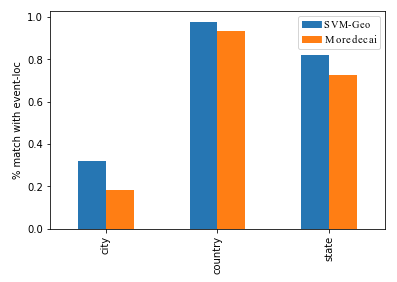
\includegraphics[width=0.6\textwidth]{figures/Geo_metrics.png}
    \caption{Performance comparison of the proposed geocoder vs state-of-the-art geo-coder Mordecai}
    \label{fig:geoPerformance}
\end{figure}

Our geocoding model works by first extracting all named entities namely Locations, Organizations and Person names, from text. We then query an elasticsearch database of Geonames for all possible expansions of a location entity mention. Once all possible expansions for a mention is obtained, we then decide which among the expansions is referred to in the text. This process is called Geo disambiguation. Most of the existing state-of-the-art methods like Kamalloo, et al. rely on hand-coded rules/hypotheses, e.g., location names mentioned consecutively share a common ancestor, names only refer to the most populous expansion, etc., for disambiguating location names.  Unlike these methods, we try to learn the rules automatically using machine learning. For each location expansion we built a feature set based on its frequency, the corresponding country and state frequency, distance to nearest mention of the corresponding country/state (both before and after), relative population of this expansion with respect to others etc. These features are then fed into a Random Forest classifier to decide which location a given named entity refers to. Since we do not use any features based on the words in the text, our method is language agnostic unlike other supervised geo disambiguation methods like Mordecai. Mordecai makes use of the words/context around a named entity mention to identify the country. We also query the organization names obtained to see if it mentions a country or state (for example, the entity “Indian Department of Treasury” gives hint about the country India). 

\section{Actor/Target Linking}
In this section we identify how entities in text identified as subject/object are converted/linked to actors of interest for our purpose. Proper nouns or entities recognised as \\
PERSON/ORGANIZATION during the language enrichment step are first checked against the list of known Actors and their aliases. We specifically make use of Jaccard similarity (in terms of words/terms instead of characters) to identify the best match.  If an entity recognised by the NER system is not found in our list of known actors we call the actor as “Unknown” and also mark it for human supervision.

For text detected as subject or generic nouns, e.g., hospitals, military, etc., we make use of wordnet to identify their semantic category and use the identified semantic category as the final detected actor if it's in our generic actors list (generic actors list includes actors/targets like military, terrorists, buildings, people etc.).

\section{Temporal Reasoning}
In this step, we build techniques to understand which date the event occurred. For this, first we make use of Heideltime~\cite{heideltime} temporal tagger for resolving any date/time mentions in the text. Heideltime supports innumerous languages and has exhaustive set of patterns for identifying mentions of relative temporal expressions and resolving them with respect to anchor date. The anchor date in our case is taken to be the article publication date if this information is available (in the meta tags) else it is assumed to be the date at which the article was crawled.

\section{Sub-type Identification}
For sub-type identification we make use of word-net and word-embedding based similarity measures with respect to the domain keywords.

\section{Event De-duplication}
Once an event is extracted from an article, we need to identify if the event refers to already extracted event in the database. If it refers to an already extracted event, then the current event is a duplicate and will be discarded. This entire process is called event de-duplication. In our framework, we perform de-duplication by comparing the source article text with the article text of all events within the last 2 days and deem it to be a threshold if the article similarity is higher 0.8. The article similarity is calculated as a weighted sum between 1) entity similarity, 2)location similarity and 3) text similarity. Text similarity is calculated using cosine similarity. While entity and location similarity are calculated using Jaccards metric~\cite{jaccard}.
\section{Experimental Settings and Evaluation}
All models, unless otherwise stated, are trained on data up to May 2018. Data from June 2018 is used for validation. The results are reported on the remaining months, i.e., August through October 2018. Note, Nov-Jan 2019 is not used for evaluation as these months only have ground-truth for Military Action events.

As stated in the previous sections, the machine learning models perform five micro-tasks in total - Event Detection, location identification, actor/target extraction, event-subtype identification, date extraction. For all micro-tasks, except for date extraction, the ML models can abstain from making a prediction. In such cases the document is sent for human supervision and the annotators are asked to provide an answer for that micro-task. Note the annotators only fill-in the information for the asked field (as defined by the micro-task) and do not change any other fields extracted by the ML models.

We report the performance of our overall system using the Performance metrics as defined by the IARPA OSI Mercury program. The performance metrics include -  
\begin{itemize}
    \item \textbf{Event Detection Performance Metrics}
    \begin{itemize}
        \item Precision/Recall/F1 metrics: These metrics are defined as expected and are standard.
\item Risk-Coverage Curve: Risk is defined as the percentage of false classifications (False Positives + False Negatives) w.r.t to the number of data points that are considered / covered. Coverage is defined as the percentage of data remaining after churning out documents on which the model score is less than the identified threshold. The curve is plotted by first sorting the model predictions in terms of its confidence score and moving the threshold from 0 to 100th percentile value of the confidence score. 
    \end{itemize}

\item \textbf{Event Encoding Performance Metrics}
    \begin{itemize}
        \item \textbf{Quality Score:} A score out of 4 and is a weighted sum over the extraction performance for each individual field in an event record. The performance for each field is a score between 0 and 1, with 1 indicating perfect extraction and 0 referring to fully wrong extraction. The components of QS are  
        % \textcolor{red}{Need to explain each individual score metric}
            \begin{enumerate}
                \item Actor score
                \item Target Target score
                \item Target Status score
                \item Location score
                \item Event Sub-type score
                \item Date score
            \end{enumerate}

         \item \textbf{Macro and Micro averages:} The macro and micro averages of the 
    above mentioned metrics are defined similar to the macro and micro averages in classification problems. For Macro-average, we first calculate QS, Precision, Recall and F-1 per document (i.e. the extracted events in a document are only evaluated against the ground-truth events in that document) and then take the average of the scores per document. 
    For Micro-average metrics, we evaluate all extracted events against all ground-truth events irrespective of which document they came from.
    \end{itemize}
\end{itemize}

\section{Results and Discussion}
In this section we will present the scores obtained by our event encoding system. Specifically we aim to answer the following major questions.

\begin{enumerate}
    \item What is the event detection performance of our AutoGSR system?
    \item How good is the uncertainty/confidence characterization of the event detection model?
    \item What is the performance of human annotators for each micro-task?
    \item How many documents are abstained per micro-task?
    \item What is the event extraction performance of the ML only System?
    \item What is the event extraction performance of the Hybrid System?
    \item What is the overall conclusion for performing MANSA event encoding?
    % \item What is the performance of our system in CU event encoding?
\end{enumerate}
In the following subsections we will look at each question individually.

\subsection{What is the event detection performance of the ML-only system?}
Here we present the performance of our ML system for the micro-task of event detection. The event detection micro-task involves predicting if an article contains an event or not. 

\begin{table}
    \centering
   \begin{tabular}{lrrrr}
\toprule
{} &  Precision &  Recall &    F1-score &  Support \\
\midrule
No-event            &  0.97 &   0.95 &  0.96 &   15843 \\
Event               &  0.75 &   0.84 &  0.79 &   2760 \\
micro avg           &  0.93 &   0.93 &  0.93 &   18603 \\
macro avg           &  0.86 &   0.90 &  0.88 &   18603 \\
weighted avg        &  0.94 &   0.93 &  0.94 &   18603 \\
\bottomrule
\end{tabular}
    \caption{Event Detection performance for English documents in test set.}
    \label{tab:engDetection}
\end{table}


\begin{table}
    \centering
   \begin{tabular}{lrrrr}
\toprule
{} &  Precision &  Recall &    F1-score &  Support \\
\midrule
No-event            &  1.0 &  1.00 &  1.00 &  28643 \\
Event               &  1.0 &  0.36 &  0.53 &   73 \\
micro avg           &  1.0 &  1.00 &  1.00 &  28716 \\
macro avg           &  1.0 &  0.68 &  0.76 &  28716 \\
weighted avg        &  1.0 &  1.0  &  1.00 &  28716 \\
\bottomrule
\end{tabular}
    \caption{Event Detection performance for Arabic documents in test set.}
    \label{tab:arDetection}
\end{table}

The tables Tab.~\ref{tab:engDetection} and ~\ref{tab:arDetection} provides the performance metrics our event detection system for English (Tab.~\ref{tab:engDetection}) and Arabic documents (Tab.~\ref{tab:arDetection}) for the test period.

We note that the performance of event detection is better in English than Arabic. However, it is to be noted that for Arabic, the event detection task is extremely imbalanced (the ratio of positive documents is 0.2\% vs 14.8\% for English). 


\subsection{How good is the uncertainty/confidence characterization of the event detection model?}
As mentioned above, the confidence score of  the event detection is taken to be the predicted probability of the max class. Figure.~\ref{fig:engPrec} gives the precision vs confidence plot for English documents and Figure.~\ref{fig:arPrec} for Arabic documents.

\begin{figure}
    \centering
    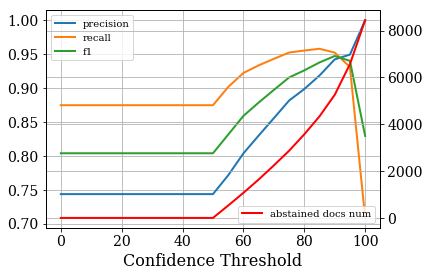
\includegraphics[width=0.6\textwidth]{figures/english_precConf.png}
    \caption{Precision vs Confidence plot for English. The right-side axis denotes the number of documents that will be abstained at the current threshold}
    \label{fig:engPrec}
\end{figure}

\begin{figure}
    \centering
    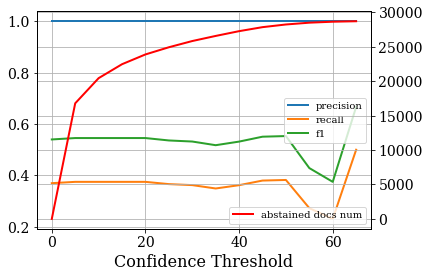
\includegraphics[width=0.6\textwidth]{figures/arabic_precConf.png}
    \caption{Precision vs confidence plot for Arabic}
    \label{fig:arPrec}
\end{figure}

From Figure.~\ref{fig:engPrec}, we can see that Precision, Recall, F-1 metrics increase almost uniformly as the confidence threshold is increased. The Recall and F-1 metrics fall sharply for high values of the threshold.
However for Arabic (From Figure.~\ref{fig:arPrec}), there isn’t much performance improvement achieved by thresholding on the confidence.

Another way at quantifying uncertainty of the classification model would be to look at the area under the Risk-Coverage (RC) curve. Figure.~\ref{fig:engRisk} provides the RC curve for English and Arabic.
\begin{figure}
    \centering
    \begin{subfigure}[b]{0.45\textwidth}
         \centering
         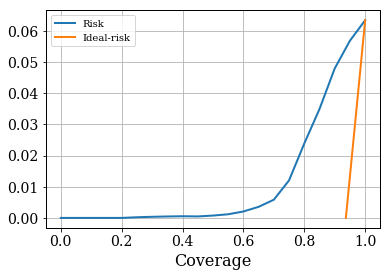
\includegraphics[width=\textwidth]{figures/english_riskCoverage.png}
         \caption{}
         \label{fig:engRisk}
    \end{subfigure}
    \hfill
    \begin{subfigure}[b]{0.45\textwidth}
         \centering
         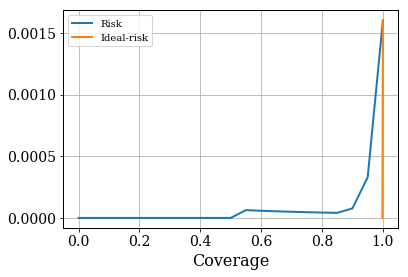
\includegraphics[width=\textwidth]{figures/arabic_riskCoverage.png}
         \caption{}
         \label{fig:y equals x}
     \end{subfigure}
     \caption{Risk-coverage curve for (a) English and (b) Arabic. The orange curve represents the ideal-risk i.e., the risk when the classifier is correctly calibrated
 ($\textrm{loss}(x_i) > \textrm{loss}(x_j) \textrm{, iff conf}(x_j) < \textrm{conf}(x_i))$}
\end{figure}

We notice from Figure.~\ref{fig:engRisk} that the risk drops to almost zero at about 50\% coverage. Note Risk is defined as the percentage of False classifications.



\subsection{What is the performance of human annotators for each micro-task?}
For estimating the performance of each human annotator, we randomly chose a micro-task for a given document and asked the annotator to provide encoding for the field denoted by the micro task. For each micro-task, the annotators were shown the encoding of the remaining fields, however they were not allowed to change these fields.

The pie chart shown in Figure.~\ref{fig:microTimings} gives the time distribution (in seconds) per micro-task. The time per task reported here is the average of the median time taken by each annotator. The median is taken after removing the top and bottom 10 percentile of times of an annotator. This is done to remove anomalous records (For example, cases where the annotator simply leaves the autogsr web-page on without logging off.)

\begin{figure}[h!]
    \centering
    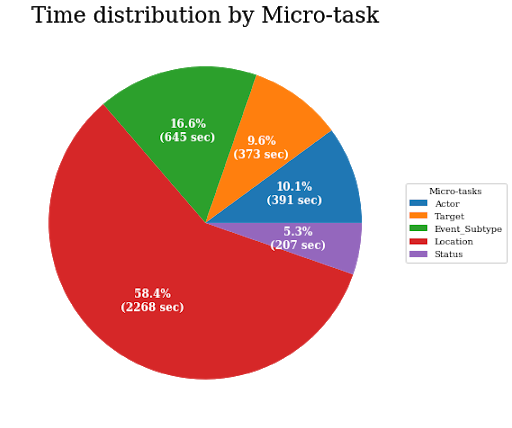
\includegraphics[width=0.5\textwidth]{figures/micro_task_timings.png}
    \caption{Average time spent per document per microtask by an annotator}
    \label{fig:microTimings}
\end{figure}

Figure.~\ref{fig:microTimings} shows the human annotators spent maximum time (58.4\%, ~approx 37 minutes) in encoding the location of the events. The least amount of  time was spent on  identifying the status of the article. Note status here refers to the event detection task.  The average accuracy per micro-task across all annotators is provided in Figure.~\ref{fig:microPerf}. We can see that the annotators have difficulty in identifying the status of an article.


\begin{figure}[h!]
    \centering
    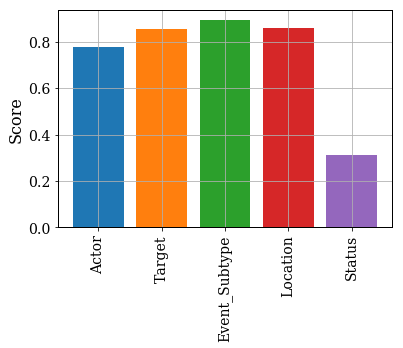
\includegraphics[width=0.5\textwidth]{figures/micro_task_performance.png}
    \caption{Average accuracy of human annotators on micro-tasks}
    \label{fig:microPerf}
\end{figure}

\subsection{How many documents are abstained per micro-task by the ML system?}
\begin{table}[]
    \centering
    \small
    \begin{tabular}{l|r}
    \toprule
       \textbf{Micro-Task}  & \textbf{\#Abstained Documents} \\
    \midrule
       Event Detection &  1936 / 57401 (3.00\%) \\
       Location  & 307/2137 (14.3\%) \\
       Actor/Target & 1002/2137 (46.8\%) \\
       All (Location, Actor, Subtype) & 320/2137 (14.9\%) \\
    \bottomrule
    \end{tabular}
    \caption{Documents sent for human supervision}
    \label{tab:abstPerMicro}
\end{table}



In this section we discuss the number of documents the ML system abstained from making a prediction for each micro-task. The threshold for abstention for different micro-tasks was identified based on the validation set performance.  The threshold for event detection for Table.~\ref{tab:abstPerMicro} summarizes the number of documents we sent for human supervision for each micro-task

\subsection{What is the event coding performance of the ML only System?}
\begin{table}
\centering
\begin{tabular}{l|r|r}
\toprule
             Metrics &    Macro-avg &    Micro-avg \\
\midrule
               \#docs &   888 &   888 \\
 \# GroundTruthEvents &  2039 &  2039 \\
   \# ExtractedEvents &  1981 &  1981 \\
         Actor Score &     0.373888 &     0.602880 \\
          Date Score &     0.940764 &     0.840740 \\
 Event Subtype Score &     0.449895 &     0.680532 \\
      Location Score &     0.866620 &     0.800837 \\
 Target Target Score &     0.662297 &     0.677204 \\
 Target Status Score &     0.590778 &     0.828618 \\
           Precision &     0.691522 &     0.949447 \\
              Recall &     0.720177 &     0.891757 \\
       Quality Score &     2.774264 &     2.999131 \\
\bottomrule
\end{tabular}
\caption{Performance metrics of ML only system}
\label{tab:mlPerformance}
\end{table}
The table.~\ref{tab:mlPerformance} provides the quality scores of the events extracted from the machine learning model in the un-abstained set  (i.e from documents that are not sent for human supervision). Note we score events extracted from a document only against the ground-truth events from that document. For overall precision and recall we average precision and recall for each individual document. 

We can see from Table.~\ref{tab:mlPerformance} that the ML only system is very good at location and date extraction. The system does not perform well on  Actor identification. On further investigation of the events extracted by the ML system we found that the ML system is not able to distinguish between the different state actors of a given country. For example, ML model is not able to differentiate between “Iraqi Special Forces” and “Iraqi Security Forces” or “Iraqi Intelligence Service”.  We thus performed another evaluation after combining all state actors belonging to a country into a single entity. That is, we group all state actors of a country like “Iraq Security Forces”, “Iraqi Intelligence Service” , “Iraqi Police”, “Baghdad International Airport Security”, “Iraqi Military” and “Iraqi Special Forces” into one single entity  “Iraqi State Actors”.  The performance of our system after this correction is shown in Table.~\ref{tab:mlgrouped}.
\begin{table}
\centering
\begin{tabular}{lrr}
\toprule
              Metric &    Macro-avg &    Micro-avg \\
\midrule
               \#docs &   888 &   888 \\
 \# GroundTruthEvents &  2039 &  2039 \\
   \# ExtractedEvents &  1981 &  1981 \\
         Actor Score &     0.551631 &     0.727570 \\
          Date Score &     0.940403 &     0.842904 \\
 Event Subtype Score &     0.451160 &     0.682170 \\
      Location Score &     0.867125 &     0.805017 \\
 Target Target Score &     0.588879 &     0.677740 \\
 Target Status Score &     0.661664 &     0.822260 \\
           Precision &     0.691522 &     0.951026 \\
              Recall &     0.720177 &     0.893247 \\
       Quality Score &     2.892902 &     3.087752 \\
\bottomrule
\end{tabular}
\caption{Performance metrics of ML only system with different state actors of one country grouped into one entity}
\label{tab:mlgrouped}
\end{table}


\subsection{What is the event coding performance of the hybrid system?}
\begin{table}[]
    \centering
    \begin{tabular}{lrr}
\toprule
              Metric &    Macro-avg &    Micro-avg \\
\midrule
               \#docs &  2137 &  2137 \\
 \# GroundTruthEvents &  4265 &  4265 \\
   \# ExtractedEvents &  4239 &  4239 \\
         Actor Score &     0.621032 &     0.755090 \\
          Date Score &     0.952899 &     0.878390 \\
 Event Subtype Score &     0.539359 &     0.646776 \\
      Location Score &     0.926107 &     0.838040 \\
 Target Target Score &     0.680881 &     0.703337 \\
 Target Status Score &     0.727046 &     0.828054 \\
           Precision &     0.791948 &     0.946720 \\
              Recall &     0.819668 &     0.915887 \\
       Quality Score &     3.121909 &     3.161470 \\
\bottomrule
\end{tabular}
    \caption{Performance metrics of the hybrid system for MANSA Event Encoding}
    \label{tab:hybridPerf}
\end{table}
Table.~\ref{tab:hybridPerf} provides the event extraction performance for the Hybrid system. The hybrid system includes predictions from the ML system along with inputs from human annotators for the micro-tasks on documents where the ML system was not confident on.


\subsection{What is the overall Conclusion for creating a MANSA event encoding system?}
From Tables.~\ref{tab:mlPerformance} and ~\ref{tab:mlgrouped} we can see that the ML models performs well in identifying Location, Date, and event status as compared to the human annotators. The human annotators on average perform better than the ML model on Actor and Target identification. 
A viable system could be one where the ML system performs the location, date and status identification and human annotators provide the actor/target extraction. The human annotators on average take approximately 12.6 minutes per document for actor and target identification and have an accuracy of approx ~80\% for the extraction of the two fields.  So for a dataset similar to our test set, we would need approximately 448.77 man hours.


% \subsection{What is the  performance of our system in CU event encoding?}
% For Civil Unrest, we train all our models on data obtained from the EMBERS autogsr system. And for testing we use the CU event articles from the CFA dataset. This experimental setting was chosen due to the presence of only a few articles with CU events in the CFA dataset.

% Table 8 provides the event detection performance for Civil Unrest. 


\section{Conclusion}
We have presented an event encoding system for Military Action and Non-state actor events as well as for Civil Unrest events. Specifically we built a system to minimize human effort and to judiciously decide suitable human-machine combinations to yield high performance. The  innovative aspects of our system are as follows:
\begin{itemize}
    \item Hybrid Event encoding wherein the machine learning system decides for which documents and which fields human supervision is required.
    \item State-of-art Geocoding, wherein location entities in an article are disambiguated based on a language independent supervised classification engine.
    \item Effective uncertainty estimation for text classification using Metric learning and Dropout based ensemble modeling.
    \item Unsupervised rule based extraction of semantic information of type \textless \textit{actor, target, type, location, date}\textgreater~from text using universal dependency parsing and multilingual wordnet.
\end{itemize}



.

\bibliographystyle{abbrv}
\bibliography{references.bib}
\end{document}
\endinput
%%
%% End of file `sample-authordraft.tex'.
